%By: Héctor Fernando Carrera Soto
%hfcarrerasoto.usac@ingenieria.usac.edu.gt

\documentclass[12pt,letterpaper, onecolumn, titlepage, oneside]{book}
%\usepackage[utf8]{inputenc}
\usepackage[spanish]{babel}

%Codificación de Fuente, permite usar tildes directamente, sin ningún tipo de error.
\usepackage[T1]{fontenc}


\usepackage{amsmath}
\usepackage{amsfonts}
\usepackage{amssymb}
\usepackage{graphicx}
\usepackage[left=2.5cm,right=1.5cm,top=1.5cm,bottom=1.5cm]{geometry}

%Para tachar dimencionales usar \cancel
\usepackage{cancel}

%>>>>>>>>>>>>>><Fuente parecido al arial<<<<<<<<<<<
\usepackage{helvet}
\renewcommand*\familydefault{\sfdefault}



\usepackage[pdftex]{hyperref}


%<<<<<<<<< para saltos de página usar  \clearpage >>>>>
%<<<<<<<<< para saltos entre líneas usar \vspace{2cm}>>>>>
%<<<<<<<<< para espaciado horizontal \hspace{1cm}>>>>>
%<<<<<<<<< para colocar url o referencias a url usar \url{http://www.latex-project.org/} o  \href{http://www.latex-project.org/}{latex project}>>>>>>>}

%Texto al azar
\usepackage{lipsum}

%Arreglar figuras



%Sangría
\setlength{\parindent}{0pt}
\usepackage{cancel}
\spanishdecimal{.}


%\frontmatter Se supone que se refiere a las partes previas al cuerpo del libro propiamente dicho: prólogo, introducción, índices. Si introducimos ese comando al principio del fichero haremos que las páginas se numeren en números romanos y que el comando \chapter no incluya el número ni la palabra "Capítulo" (como ocurriría si usáramos \chapter*), pero sí incluya el título en el índice (cosa que no ocurriría de usar \chapter*).

%\mainmatter Con este comando le indicamos a LaTeX que ha terminado la parte inicial y a continuación viene el libro propiamente dicho. Hay que usarlo cuando se ha usado previamente \frontmatter. El efecto de \mainmatter es que se reinicia la numeración de las páginas, que pasan además a volver a numerarse con números arábigos. El comando \chapter vuelve además a su comportamiento habitual.

%\backmatter se debe usar (si se usa) al final del documento. Provoca que \chapter funcione igual que en \frontmatter, pero no afecta a la numeración de las páginas.

\usepackage{enumerate}

\begin{document}

%-----------Caratula no tocar--------------------
\newcommand{\HRule}{\rule{\linewidth}{0.2mm}}

\begin{titlepage}
\begin{center}

\vspace{0.5cm}

{\Huge Universidad de San Carlos de Guatemala}

\vspace{1cm}


{\large Facultad de ingeniería.}\\
{\large Escuela de ingeniería mecánica eléctrica.}


\vspace{0.5cm}


0230 - Instrumentación eléctrica.\\
Sección O.


\vspace{0.5cm}

\begin{figure}[h]
\centering

\includegraphics[scale=0.8]{logo-fiusac.png}
\end{figure}

\vspace{0.5cm}

		
\HRule \\[0.4cm]
{ \huge \bfseries Instrumentación virtual
}\\[0.4cm]
\HRule \\[1.5cm]

\begin{tabbing}
\hspace{4cm}\=\hspace{7.5cm}\=\kill
\>  Nombre: \> Carné:\\
 \>  Héctor Fernando Carrera Soto \> 201700923 \\ 
 \>  Gerson Alexander Cux Garcia \> 201700635 \\ 
 \>  Francisco Javier Santos Gonzáles \> 201709393 \\ 
 \>  Josué Daniel Reyes Mendizabal \> 201709387 \\ 
 \>  Luis Alfredo Reyes Chávez \> 201700903
\end{tabbing}  

\vspace{0.5cm}

\textbf{{\large 29 de junio de 2021}}
		
\end{center}
\end{titlepage}


%-----------------Indice--------------------------
\tableofcontents
\clearpage

%-------------------Introducción----------------------
% \frontmatter reinicia la enumeración de todas las páginas
\frontmatter

\chapter{Introducción}
La instrumentación es un grupo de elementos que ayudan en la interacción hombre-maquina, cuyo uso es específicamente para medir, convertir, transmitir, controlar y registrar las variables que presentan los procesos, esto con el objetivo de generar una optimización de los recursos que se están utilizando. Aplicando conocimientos de química, mecánica, electricidad, electrónica e informática.\\

Debido a la constante actualización de los sistemas de procesos de control, la instrumentación ha tenido que evolucionar al mismo ritmo que lo hace la industrializaciones de las cosas, permitiendo que se lleven mejor los procesos de control. La instrumentación eléctrica afronta ahora el reto de la digitalización de las cosas, la cual ha llevado la necesidad de la evolución de esta nuevamente, implementando nuevas metodologías de control y medición enfocadas a  la virtualización de los sistemas ciberfísicos y la robótica.\\

En base a este constante crecimiento de la instrumentación, se presenta el siguiente trabajo escrito el cual contiene una breve historia de como a trascendido la instrumentación desde sus orígenes hasta la actualidad, también se menciona sobre las nuevas técnicas de instrumentación debido a la virtualización de los procesos de control, así también los lenguajes de programación y protocolos de la comunicación de la nueva instrumentación y el futuro de la instrumentación eléctrica debido a las tendencias actuales.

%-----------------------------------------------
%-----------------------------------------------
%-------------------Inicio cap 1-----------------------
\mainmatter
\chapter{Marco conceptual}
%-----------------------------------------------
\section{Evolución de la instrumentación }
Los procesos industriales exigen el control de la fabricación de los diversos productos obtenidos. Los procesos son muy variados y abarcan muchos tipos de productos: la fabricación de los productos derivados del petróleo, de los productos alimenticios, e industria cerámica, las centrales generadoras de
energía, la siderurgia, los tratamientos térmicos, la industria papelera, la industria textil, etc.\\

En todos estos procesos es absolutamente necesario controlar y mantener constantes algunas magnitudes, tales
como la presión, el caudal, el nivel, la temperatura, el PH, la conductividad, la velocidad, la humedad, el punto
de rocío, etcétera. Los instrumentos de medición y control permiten el mantenimiento y la regulación de estas
constantes en condiciones más idóneas que las que el propio operador podría realizar.\\

En los inicios de la era industrial, el operario llevaba a cabo un control manual de estas variables utilizando sólo instrumentos simples, manómetros, termómetros, válvulas manuales, etc., control que era suficiente por la relativa simplicidad de los procesos. Sin embargo, la gradual complejidad con que éstos se han ido
desarrollando ha exigido su automatización progresiva por medio de los instrumentos de medición y control.\\

\subsection{Orígenes de la instrumentación}
\begin{itemize}
    \item Los inicios de los años 20 y 50, se dio el desarrollo formal de la instrumentación por los requerimientos de los nuevos procesos industriales, tales como la refinación del petróleo, la pasteurización de los lácteos o la generación de electricidad.
    \item Antes de 1920. Las mediciones se efectuaban localmente. Los Sistemas de Instrumentación y Control eran dispositivos manuales mecánicos y no existía la transmisión. Todo se realizaba con el operador trabajando junto al proceso. No existían métodos formales ni modelos matemáticos para poder controlar las variables: predominaban los métodos heurísticos, mediante la prueba y el error o la causa y el efecto.
    \item De 1930 a 1940. Continuó la evolución de sistemas más confiables. Se construyeron los primeros servomecanismos, se utilizaron los primeros dispositivos neumáticos y se desarrollaron los primeros analizadores. Con respecto a los Sistemas de control, se desarrollaron los primeros controladores industriales que utilizaron aproximaciones a los algoritmos Proporcional-Integral-Derivativos (PID).
    \item De 1930 a 1940. Continuó la evolución de sistemas más confiables. Se construyeron los primeros servomecanismos, se utilizaron los primeros dispositivos neumáticos y se desarrollaron los primeros analizadores. Con respecto a los Sistemas de control, se desarrollaron los primeros controladores industriales que utilizaron aproximaciones a los algoritmos Proporcional-Integral-Derivativos (PID).
    \item Entre los años 1940 y 1950. Las plantas alcanzaron grandes capacidades de producción, su tamaño y complejidad aumentaron. En este periodo se desarrollaron los primeros instrumentos electrónicos, basados principalmente en potencias. Se construyeron los primeros transmisores y las primeras celdas de presión diferencial.\\
\end{itemize}

\subsection{Desarrollo de la instrumentación}
 El desarrollo se inició con los manómetros, termómetros y válvulas manuales localmente montados. En esta fase eran necesarios muchos operadores para observar los instrumentos y maniobrar las válvulas. Los procesos y los instrumentos eran proyectados empíricamente basándose en la intuición y en la experiencia acumulada y no estaban centralizados para conseguir una mayor eficiencia en las funciones del operador.\\
 
 La siguiente etapa fue la centralización de las funciones de medida y de control más importantes, pertenecientes a una operación del proceso, en un panel localmente montado. De este modo podía observarse y controlarse el funcionamiento de cada elemento particular de la instalación de una manera
más coordinada y eficaz. Para hacer esto posible, se desarrollaron instrumentos galvanométricos operados por termopar, termómetros con largos capilares y caudalímetros con largos tubos de conducción de la presión diferencial.\\

A medida que pasó el tiempo, estas salas de control se hicieron indebidamente grandes, debido al crecimiento de los procesos y al tamaño de los instrumentos convencionales y se desarrolló la instrumentación neumática miniatura que apareció en el mercado hacia el año 1947, dotada ya con conmutación automático-manual incorporada, pero con el mismo tipo de transferencia.\\

Los complejos de múltiples procesos empezaron a utilizar salas de control separadas y la coordinación y la comunicación entre los operadores en estas salas de control comenzaron a plantear algunos problemas. Además se introdujeron equipos centrales de tratamiento de datos que requerían la disponibilidad de diversas señales de medida en un punto central. \\

Los paneles de alta densidad permitieron básicamente que un operador supervisase un gran complejo compuesto por muchos procesos.\\

Los sistemas de instrumentación de alta densidad normalizaron sus dimensiones a 6 X 3" (150 X 75mm) en indicadores controladores y 6 X 6" (150 X 150 mm) en registradores, y tuvieron que satisfacer los siguientes requisitos básicos e importantes:\\

\begin{itemize}
    \item Permitir que el operador asimile rápidamente la información.
    \item Permitir que el operador tome sus decisiones muy rápidamente.
    \item Permitir una rápida ejecución de las decisiones del operador. 
\end{itemize}

La primera característica la proporcionó el indicador de desviación, que facilita tres elementos de información:\\

\begin{itemize}
    \item La existencia de una desviación. 
    \item Si la desviación es positiva o negativa.
    \item Cuál es la magnitud de la desviación. 
\end{itemize}

En 1983 aparece el transmisor digital inteligente con señal de salida analógica de 4-20 mA c.c. y se inicia el desarrollo de las comunicaciones (field bus) entre los instrumentos del lazo de control. Se eliminan las incómodas y caras calibraciones necesarias en los instrumentos convencionales y se facilita
el cambio del campo de medida y el auto-diagnóstico. En 1986 aparece el primer transmisor enteramente digital con lo que aumentan todavía más las prestaciones, con la única limitación importante en la normalización de las comunicaciones donde todavía no es posible el intercambio de instrumentos de diferentes marcas.\\

Cabe también señalar que se están aplicando técnicas de análisis en la interfase hombre-máquina en la seguridad y fiabilidad de operación de sistemas complejos. Estas técnicas se iniciaron en el campo de las centrales nucleares, en aviación y en sistemas informáticos. Estos estudios, cuyo objeto es analizar los incidentes y los accidentes ocurridos (por ejemplo, la catástrofe de Chernobil en Rusia) y poner los medios oportunos para que los errores humanos y técnicos que los han causado no vuelvan a presentarse, han iniciado sus aplicaciones en las plantas de proceso. 

Las técnicas que utilizan son en general: 
\begin{itemize}
    \item Cadenas de Markov, que definen un proceso aleatorio en un cierto número de estados finitos probables. 
    \item Análisis de fallos en Arbol (fault-tree analysis) que ante un suceso (fallo de un equipo o error humano) proporciona la secuencia cronológica de accidentes que pueden tener lugar. 
    \item  Simulación de Monte-Carlo, que permite la estimación del tiempo de fallo de un sistema a partir de las funciones de densidad de probabilidad de sus componentes individuales. 
    \item Técnica Dylam, que modeliza los componentes del sistema, define los algoritmos de control, establece los sucesos de partida (por ejemplo, búsqueda de sucesos que puedan provocar temperaturas elevadas en el proceso) y genera y analiza los sucesos. 
    \item Modificación de la fiabilidad humana (razonamiento ante incertidumbre, error humano ante tiempos límite de reacción y factores humanos). 
    \item Fiabilidad del software.
\end{itemize}

\subsection{Puntos Finales}
La industria está considerada por los economistas como uno de los grandes valedores del crecimiento económico. Lo cierto es que es el sector que genera más valor añadido (aplicación de nuevas tecnologías, innovación, trabajadores especializados) y también aporta mayores retribuciones a los trabajadores. Además, es el gran motor exportador. Aragón ha experimentado en el comienzo del siglo XXI un crecimiento exponencial que, de momento, ha alcanzado su cota más elevada en el segundo trimestre de este año, con un alza del 5\%. El pasado año alcanzó un alza del 3,7\%, mientras que en los años precedentes la industria llegó a bajar de un crecimiento del 1\%.\\

A lo largo de la primera y la segunda revolución industrial de la innovación mecánica y la producción en masa, la instrumentación y su desarrollo fueron una tecnología clave de apoyo. Los desarrollos de instrumentos a nivel sensor han involucrado tanto al sector mecánico como al químico, mientras que la transmisión de valores ha hecho uso de las industrias electrónicas forjando los avances a través de la tercera industrial usando electrónica y avanzar para avanzar en el análisis del procesamiento de datos de señal. A medida que entramos en el período apodado la cuarta revolución industrial, Inteligencia Artificial, Grandes Datos y más.\\

La instrumentación debe participar en un mundo de datos digitales y análisis forenses para enfrentar los desafíos y las expectativas de esta cuarta revolución industrial.\\

\begin{center}
    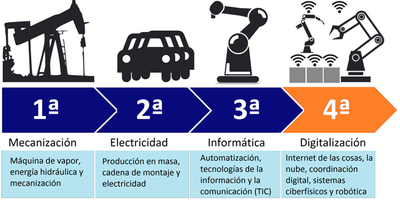
\includegraphics[scale= 0.8]{avance.png}
\end{center}



%-----------------------------------------------
\section{Lenguajes de programación virtual}
Hoy en día se tienen varios lenguajes de programación los cuales pueden utilizarse para desarrollar aplicaciones de instrumentación virtual en diferentes áreas de estudio. Estos lenguajes tienen en común el hecho de que se basan en conjuntos de instrucciones de texto creando líneas de código. Como ejemplos de estos lenguajes se tienen: C/C++, C\#, Java, Phyton, por mencionar los más utilizados. Dichos lenguajes ofrecen diferentes ventajas y desventajas entre sí, las cuales
permiten el desarrollo de interfaces virtuales aplicables a la instrumentación.

\begin{center}
    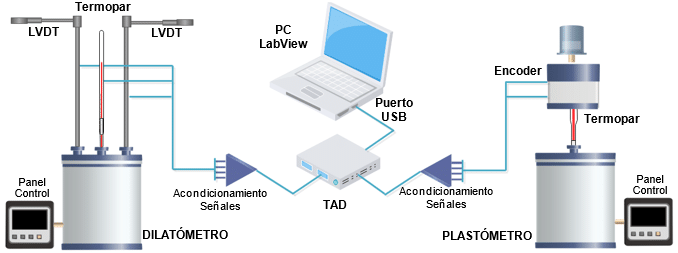
\includegraphics[scale=0.6]{VIRTUAL.png}
\end{center}

Sin embargo, la instrumentación virtual se basa en la interacción del usuario con interfaces computacionales gráficas para el control y monitoreo de sistemas físicos, por lo cual los lenguajes gráficos ofrecen mayores ventajas respecto a los lenguajes tradicionales basados en texto (Goldberg, 2000). El lenguaje gráfico —también llamado lenguaje G— más utilizado para
desarrollar aplicaciones de instrumentación virtual es el LabVIEW® (Laboratory Virtual Instrument Engineering Workbench) desarrollado por la empresa National Instruments en 1986, el cual elimina múltiples detalles sintácticos asociados con los lenguajes basados en texto, ya que se trata de un modelo de programación gráfica con el cual se tienen diferentes ventajas en relación a los lenguajes mencionados anteriormente. Por esta razón, se ha constituido, en la actualidad, como el
estándar para aplicaciones de instrumentación virtual (National Instruments, 2011).
\\
\\
Los códigos gráficos incluyen una interfaz de usuario completamente gráfica y un código fuente basado en el uso de bloques de conexión interconectados mediante cables. La creación de los lenguajes de programación gráfica, y su inherente evolución, ha permitido el desarrollo de múltiples protocolos e interfaces de comunicación creados con el objetivo de abarcar una amplia gama de aplicaciones industriales programables en lenguaje gráfico, lo cual ha constituido la base
de la instrumentación virtual.

%-----------------------------------------------
\section{Buses y protocolos de comunicación en instrumentación virtual}

\subsection{Instrumentación Virtual}

Antes de saber cuales son los buses y protocolos de comunicación en la instrumentación virtual, debemos saber, que es la instrumentación virtual. Bien la instrumentación virtual  es el uso de software personalizable y hardware de medición modular para crear sistemas de medición definidos por el usuario, llamados instrumentos virtuales. En donde en donde vemos que la instrumentación virtual va más allá de la simple medición de corriente o voltaje. También involucra el procesamiento, análisis, almacenamiento, distribución y despliegue de los datos e información relacionados con la medición de una o varias señales específicas. Con éstas, mediante software que permitan la implementación de algoritmos de control, es factible integrar y controlar complicados procesos. Es decir, el instrumento virtual no se conforma con la adquisición de la señal, sino que también involucra la interfaz hombre-máquina, las funciones de análisis y procesamiento de señales.


\subsection{Buses y protocolos de comunicación de instrumentación virtual}

Al conocer en términos generales que es la instrumentación virtual
En la actualidad existen diferentes protocolos de comunicación utilizados para transmitir y recibir datos de múltiples dispositivos. En el ámbito de la instrumentación virtual se encuentra un conjunto de protocolos e interfaces de comunicación aplicables a la transferencia de datos entre la computadora con la aplicación virtual ejecutándose y los periféricos externos. Dichos protocolos e interfaces que podemos mencionar son:

\begin{itemize}
    \item \textbf{Sistema de Bus RS-232 DB9:} es el estándar común usado en los puertos serie. Define las propiedades eléctricas y la sincronización de las señales, así como la interpretación de las mismas, el tamaño físico y la configuración de los pines del conector. 
    
    Los ordenadores modernos rara vez tienen puertos RS-232. Bus Serie Universal (USB) ha reemplazado la tradicional interfaz RS-232. El RS-232 tiene muchos defectos en comparación con otras tecnologías posteriores como RS-422 , RS-485 e incluso Ethernet. Estas limitaciones incluyen baja velocidad de transmisión, longitud limitada del cable, fluctuaciones sustanciales de voltaje y capacidades multipunto limitadas.
    
    Sin embargo, es posible utilizar un convertidor externo USB a RS-232 o una tarjeta de expansión interna con uno o más puertos serie para conectar un dispositivo periférico serie RS-233 al ordenador. Muchas placas madre también tienen un cabezal de puerto COM que permite instalar un soporte con un puerto DE-9.

    \item \textbf{Sistema de Bus RS485:} La interfaz RS485 ha sido desarrollada, de un modo análogo a la interfaz RS422, para la transmisión serial de datos a altas velocidades y a distancias grandes. En el sector de la automatización industrial la interfaz RS485 aún está muy extendida, pero está siendo desplazada lentamente por interfaces basadas en Ethernet.
    
    Mientras la RS422 sólo permiete la conexión unidireccional de hasta 10 receptores en un emisor, la RS485 ha sido concebida como sistema de bus bidireccional con hasta 32 usuarios. Con los modernos Transceiver-ICs es posible conectar hasta 128 usuarios a un sistema de bus mediante la reducción de la carga que generan los nodos de bus.
    
    Físicamente las interfaces RS422 y RS485 varía poco, de modo que se puede utilizar los mismos módulos Transceiver para las dos interfaces. 
    
    Dado que varios transmisores trabajan en una línea común, tiene que garantizarse con un protocolo que en todo momento esté activo como máximo un transmisor de datos. Los otros transmisores tienen que encontrarse en ese momento en estado ultraohmio.
    
    La norma RS485 define solamente las especificaciones eléctricas para receptores y transmisores de diferencia en sistemas de bus digitales. La norma ISO 8482 estandariza además adicionalmente la topología de cableado con una longitud máx. de 500 metros.
    
    \item \textbf{GPIB (General Purpose Interface Bus):} GPIB es un estándar de conexión que permite la comunicación de un ordenador con instrumentos electrónicos de medida, como pueden ser generadores de funciones, osciloscopios, etc.
    
    El bus GPIB está compuesto por 16 líneas de señal y 8 líneas de tierra. Las 18 líneas de señal están divididas en tres grupos (8 líneas de datos, 3 líneas de handshake y 5 líneas de control.)
    
    \item \textbf{PXI:} PXI (PCI eXtensions para Instrumentación) es una plataforma comprobada y basada en PC para sistemas de medidas y automatización. Proporciona energía, enfriamiento y un bus de comunicación para soportar múltiples módulos de instrumentación dentro de la misma cubierta. PXI utiliza tecnología comercial de bus PCI basada en PC combinanda el paquete CompactPCI modular y robusto, así como las características clave de temporización y sincronización.
    
    El PCI-SIG (Peripheral Component Interconnect Special Interest Group) mejoró significativamente el ancho de banda del sistema cuando lanzaron la evolución de PCI con el estándar PCI Express. El PXI Systems Alliance (PXISA), el cual regula PXI, adoptó la última generación de tecnología comercial de la PC para evolucionar PXI a PXI Express. PXI Express mantiene las características de PXI para garantizar la retrocompatibilidad, proporcionando más ancho de banda, potencia, enfriamiento y características de temporización y sincronización, además de las características PXI estándares.
    
    PXI y PXI Express pueden parecer complejos con tantas características, sin embargo, estas tecnologías tienen un núcleo común: buses de comunicación de la PC principal. Los chasis PXI y PXI Express proporcionan una arquitectura conocida y familiar para el sistema de medidas y automatización del ingeniero de hoy en día.
    
    Debido a que PXI es una especificación abierta que es administrada por el PXISA, cualquier proveedor puede construir productos PXI. Para ayudar a explicar los detalles de bajo nivel de un sistema PXI, esta nota técnica describe la especificación definida por el PXISA y cómo es implementada en hardware NI PXI.
    
    \item \textbf{VXI:} Con el tiempo el bus VME ha evolucionado en forma de nuevos buses de expansión que parten de la plataforma VME. Éste es el caso de VXI (VME eXtensions for Instrumentation) que es la extensión del bus VME para instrumentación. 
    
    
    VXI nació por la necesidad de reducir el tamaño físico de los sistemas de instrumentación y actualmente es utilizado en aplicaciones de sistema de pruebas, mediación, adquisición de datos y análisis, sistemas de automatización industrial, sistemas militares y aeroespaciales. 
    
    
    En 1987 el consorcio VXI desarrolló la normativa de VXI, con el objetivo de definir un estándar para múltiples fabricantes que se dedicaban al desarrollo de tarjetas de instrumentación, que no fue aceptada por IEEE hasta 1993, como IEEE-1155. Inicialmente los miembros del consorcio fueron GenRad, Hewlett Packard, National Instruments, Racal Instruments y Tektronix, a medida que aumentó la importancia de VXI se elevó el número de miembros. Actualmente en el mercado existen más de 250 fabricantes y más de 1500 dispositivos que implementan el bus VXI. 
    
    Entre las diferencias de VME y VXI se encuentran las líneas extras para temporización y disparo, nuevos protocolos para la comunicación y la comunicación basada en mensajes (SCPI). VXI al igual que VME son tecnologías asíncronas que cuentan con una tasa de datos máxima de 160 MBytes/s, al igual que ocurre con GPIB el ancho de banda es distribuido y por tanto, dividido por el número de elementos conectados al bus. Se debe destacar la baja latencia que posee el bus VXI.


    
    
    
\end{itemize}


%-----------------------------------------------
\section{El futuro y tendencias actuales de la instrumentación virtual}

Hoy en día nos encontramos en una era digital donde la información cobra cada vez mayor importancia en nuestras vidas, una época caracterizada por el uso intensivo por las tecnologías de comunicación e instrumentación, en esta llamada, cuarta revolución industrial, se hace uso de más herramientas digitales, buscando adaptar a estas herramientas a los cambios tecnológicos, agregando nuevas funcionalidades y conectividades, enriqueciendo la parte de la instrumentación virtual.\\

Una de las tendencias más fuertes es la llamada industria 4.0, es a la realización de aplicaciones, como la posibilidad de conectarse a servidores del internet de las cosas, desarrollar instrumentación instrumental orientado a estos dispositivos del internet de las cosas.\\

Con el tiempo y desarrollo, se han obtenido herramientas que permiten realizar aplicaciones orientadas al procesamiento de imágenes, señales, telecomunicaciones, aplicaciónes de computo embebido y reconfigurable, además de eso tiene conectividad con multiples protocolos de comunicación, buses de campos que permiten enlazarnos, no solo a plc's, si no que a distintos programas como solidworks, matlab y cualquier dispositivo con protocolo de comunicación estándar.\\

Esto permite la comunicación entre un DAQ y cualquier dispositivo que utilice los puertos del sistema correspondiente, haciendo uso de los buses, como por ejemplo, las plataformas de arduino, raspberry pi.\\

Algunas antenas que se utilizan para IOT, como lo es el chip de ESP32 por ejemplo, como observamos esto va en aumento, permitiendo la diversidad de aplicaciones, gracias a esta conectividad, si se identifica un software que soporten la comunicación estándar, se pueden usar algunas aplicaciones como LabVIEW para enlaces como por ejemplo, algunas de las tendencias actuales, el análisis estadístico de mantenimiento centrado en la confiabilidad, pruebas o análisis de calidad para verificar la repetitividad de algún proceso productivo o la estandarización de la operación con la que se lleva cabo un proceso como tal o enlaces a softwares en donde se usa la representación completamente digital de una planta industrial.\\

En realidad mucha de las aplicaciones no han sido exploradas a profundidad, debido a que se encuentra a pleno auge y sus posibilidades de aplicación son enormes, por lo que aún no se a explotada por completo.\\

Uno de sus mayores usos es en centros de investigación y desarrollo tecnológico por la felicidad de adquirir un DAQ lo suficientemente adaptados a las condiciones determinados y su flexibilidad de software para el alcance de los proyectos, sin embargo en aplicaciones industriales, son rutas distintas las que se siguen, ya que debido al tiempo, se hace uso de integraciones, ya que simplemente se usan aplicaciones ya creadas previamente.\\

Esto se debe a que en el desarrollo en plantas industriales, es menor. Por ejemplo el uso de plataformas lógicos programables (PLC), muchas veces estas plataformas, inclusive para arduino, ya que a diferencia de los PLC, requieren más tiempo de desarrollo, sin embargo, ambos tienen un procesador, aunque este último se dedica más para estudiantes, acortando el tiempo de desarrollo.

%-----------------------------------------------
\chapter{Practica}
\section{Aplicaciones de la instrumentación virtual}
La instrumentación virtual toma muchas ventajas de las últimas tecnologías incorporadas en las PCs (procesadores rápidos, grandes cantidades de memoria, espacio de almacenamiento, internet, etc.) que ayuda a aumentar la flexibilidad para crear nuevas soluciones a los problemas de pruebas y diseño.\\
Al utilizar instrumentación virtual es posible reducir los costos de adquisición y mantenimiento de equipo tradicional. Una de las ventajas es la posibilidad de conectar la PC a una red y compartir los recursos entre computadoras. Esto involucra muchas áreas de conocimiento mediante las cuales se pueden realizar un sinnúmero de aplicaciones. Para realizar dichas aplicaciones se requiere la ejecución de tres etapas básicas que son:\\
\begin{itemize}
    \item Adquisición de señales
    \item Procesamiento de datos
    \item Despliegue de resultados.
\end{itemize}
Para la adquisición de señales es necesario utilizar algún método de captura de parámetros físicos en la computado. Ya que se tienen los datos en la computadora, se requiere procesar dicha información mediante el uso de algoritmos o técnicas de análisis y procesamiento de señales de acuerdo al área de aplicación requerida.\\
Dentro de los algoritmos utilizados para procesamiento de señales en un sistema se tienen:
\begin{itemize}
    \item \textbf{Análisis espectral} (transformadas, espectrogramas, Fourier, Gabor, Choi-Williams)
    \item \textbf{Filtrado digital} (FIR, IIR, adaptivos-LMS).
    \item \textbf{Métodos de ventanas} (Hanning, Hamming, Blackman, Parzen, flat top, etc)
    \item \textbf{Ecuaciones diferenciales} (Radau IIA, cash carp, Euler, Runge Kutta, Rosenbrock, Adams-Moulton)
    \item \textbf{Interpolación y extrapolación} (Polinomiales, racionales, grids, Lagrange, Hermite)
    \item \textbf{Operaciones con señales} (convolución, autocorrelación, correlación cruzada, deconvolución, decimación, normalización)
    \item \textbf{Análisis de distorisón y ruido} (SINAD, THD, potencia de espectro, densidad espectral)
    \item \textbf{Generación de señales y ruido} (Gaussiano, Bernoulli, gamma, binomial, Poison)
    \item \textbf{Probabilidad y estadística} (histogramas, momentos, media, mediana, moda, varianza, desviación estándar, correlación, percentiles, coeficientes Speraman, Kendall's Tau).
    \item \textbf{Transformadas} (Hilbert, Fourier FFT DFT, DCT, DST, Laplace, Wavelet, Waish-Hadamard, Chirp, Hartley, Dauvechies)
    \item \textbf{Integración y diferenciación} (trapezoidal, regla de Simpson, regla de Bode).
    \item \textbf{Funciones polinomiales y solución de raíces} (máximo común divisor, mínimo común múltiplo, euclideano, raíces reales, compleas, pares conjugadas).
    \item \textbf{Mediciones de amplitud y niveles} (DC, RMS, pico, promedio, trigger, duty cycle).
    \item \textbf{Optimización} (lineal, cuadrática, Brent, Golden, aproximación de Chebyshev).
\end{itemize}

Mediante la computadora se pueden utilizar gráficas, archivos de datos, hojas de cálculo, animaciones en 3D, y cualquier elemento visual que permita y facilite el entendimiento y comprensión de los datos procesados par ael usuario, para esto es el \textbf{despliegue o visualización de los datos procesados.}

Dentro de las áreas de aplicación en las cuales se utiliza la instrumentación virtual se encuentran las relacionadas con la ingeniería:
\begin{itemize}
    \item Eléctrica
    \item Electrónica
    \item Mecatrónica
    \item Mecánica
    \item Telecomunicaciones
    \item Robótica
    \item Automotriz
    \item Aviónica y aeroespacial
    \item Biomédica
    \item Biomecánica
    \item Biotecnología
    \item Ciencias computacionales
\end{itemize}


%-----------------------------------------------
\backmatter
\chapter{Recomendaciones}



\begin{itemize}


%---------
\item Que el usuario que desee implementar algún análisis de algún equipo buscar el software que cumpla con los requisitos que el necesite.
\item Es necesario concretar el aprendizaje de como ha ido evolucionando la instrumentación en el pasar de los años, ya que en base a esto se puede predecir el comportamiento que va tomando la instrumentación, y así poder confrontar los desafíos de las nuevas mecánicas que toma la instrumentación eléctrica.
\item El usuario debe leer de manera detenida primero el manual de uso para LabVIEW y así entender de mejor manera la forma de crear un proceso por medio de lenguaje G.
\item Para el correcto funcionamiento del software, se recomienda tener instalado la plataforma de computación original de casa sistema, por ejemplo JAVA, debido a que algunos software son desarrollados en dicho lenguaje. El software cuenta con una interfaz configurable por el usuario y hará uso del código, en elementos gráficos que incluye la aplicación.

\item Considerar el cambio a los instrumentos virtuales dado que estos pueden ser de mucha funcionalidad, y el costo de mantenimiento de los mismos puede ser muy bajo, el cual a lo largo del tiempo esto es de beneficio para nosotros. 

\end{itemize}





%-----------------------------------------------
\chapter{Conclusión}

\begin{itemize}
\item Se concluye que al hay diferentes software's para la recolección de datos de algunos equipos y esto puede reducir costos y mano de obra humana para su ejecución.
\item Se concluye que la instrumentación ha evolucionado de gran manera desde la era industrial, a pensar de que esta ya existía, pero por las demandas de control de procesos esta tomo mas fuerza, llegando a lo que tenemos hoy y las diferentes técnicas de control y medición en los procesos comerciales e industriales.
\item Se concluye que los lenguajes de programación virtual de instrumentación, han ayudado en gran medida a las empresas, en el sentido que los operadores interactúan de mejor manera con las máquinas, ya que tienen una interfaz más amigable para el usuario y así, poder llevar acabo tareas complejas y extensas de manera fácil y ordenada gracias al lenguaje G.

\item La instrumentación virtual proporciona la posibilidad de tener un híbrido, un instrumento físico y uno virtual, que tenga un sistema DAQ para realizar algún proceso o monitoreo, como el caso de un multímetro digital, el cual permite hacer distintos tipos de mediciones, sin embargo, algunos instrumentos tienen funciónes limitadas, dependiendo del hardware pueden medir ciertas variables, sin embargo si agregamos un algoritmo adicional, podemos medir otras magnitudes físicas, como el ángulo de fase que se puede medir entre una línea y otra, no cambiamos el hardware, pero sí las funciónes y cálculos realizados por el multímetro, implicando la adición de hardware, en el caso de instrumentación virtual se busca exactamente lo mismo, modificando el código, para añadir nuevas funciónes en la instrumentación virtual.

\item Al analizar la información, podemos decir que la adquisición de datos por medios de los protocolos y buses de comunicación de la instrumentación virtual, podemos decir que para obtener una mejor lectura o medición, se debe escoger bien, el tipo de sistema o bus que vamos a usar, dependiendo la información que vamos obtener, es mejor un protocolo que otro, como por ejemplo el GPIB es un sistema de comunicación que nos funciona muy bien en los osciloscopios o los generadores de funciones. 



\end{itemize}



\begin{thebibliography}{99}
%Las fuentes de consulta se citan en forma organizada y homogénea, tanto de los libros, de los artículos y, en general, de las obras consultadas, que fueron indispensables indicar o referir en el contenido del trabajo.


%\bibitem{} Reckdahl, K. (Versión [3.0.1]). (2006).\textit{ Using Imported Graphics in LATEX and pdfLATEX}.

%-----------------------------------------------
\bibitem{} Aplicaciones de la instrumentación virtual en la educación tecnológica. Consultado: 24 de junio 2021, [En linea].\url{http://www.redicces.org.sv/jspui/bitstream/10972/467/1/Instrumentaci%c3%b3n%20virtual.pdf}

\bibitem{} Instrumentación virtual. Consultado: 24 de junio 2021, [En linea]. \url{https://repositorio.tec.mx/bitstream/handle/11285/622433/ID355.pdf?sequence=1&isAllowed=y#:~:text=Las\%20\%C3\%A1reas\%20de\%20ingenier\%C3\%ADa\%20que,\%2C\%20automotriz\%2C\%20avi\%C3\%B3nica\%20y\%20aeroespacial.}
%-----------------------------------------------

\bibitem{} Evolución de la Instrumentación. Consultado: 27 de junio 2021, [En linea]. \url{https://ingcaicedo.tripod.com/aut/Evol_Instrum.pdf}

\bibitem{} Instrumentación virtual. Fundamentos de programación gráfica con LabVIEW. Consultado 26 de junio 2021. [En línea]. \url{https://repositorio.tec.mx/bitstream/handle/11285/622433/ID355.pdf?sequence=1&isAllowed=y#:~:text=Como\%20ejemplos\%20de\%20estos\%20lenguajes,virtuales\%20aplicables\%20a\%20la\%20instrumentaci\%C3\%B3n.}
%\bibitem{} Goldberg, H. (2000). \testit{What is virtual instrumentation? En IEEE Instrumentation and Measurement
%Magazine, 3(4), 10-13.}

\bibitem{} Historia de la Instrumentacion. Consultado: 27 de junio 2021. [En Linea]. \url{https://www.sutori.com/story/historia-de-la-instrumentacion-industrial--cxt5hP54LQocY2JdgvorwM9X}.

\bibitem{} Reckdahl, K. (Versión [3.0.1]). (2006).\textit{ Using Imported Graphics in LATEX and pdfLATEX}.

\end{thebibliography}


\end{document}

